% Provenance (never printed): cycle 4 SVT, "La planete Terre": sedimentation,
% from sediment to sedimentary rock, fossilisation, fossils and layers as a
% record of past environments; see sources/book1/PROVENANCE.md. Book 1,
% grade 7, chapter 4.
% Vocabulary guard: first chapter allowed to use "sediment"; the principles of
% relative dating (superposition, fossil succession and the rest) and "unconformity" are
% g7.5's and are not named here; fossils as evidence of evolution are the
% biology books' (one sentence of prose).
\chapter{अवसाद और जीवाश्म}\label{ch:g7:sediments-and-fossils}

एरिज़ोना (संयुक्त राज्य अमेरिका) का ग्रैंड कैन्यन औसतन \qty{1.6}{km} गहरा है। उसकी
दीवारें \omterm{def:g3:stones-pebbles-sand:rock}{चट्टान} की परतों से बनी हैं, एक के ऊपर एक, लाल, भूरी, धूसर और हल्की
पीली। सबसे ऊपरी परत, काइबाब चूना पत्थर, में रेंजर सीपियाँ दिखाते हैं: ब्रैकियोपॉड
की सीपियाँ, ऐसे जानवर जो किसी \omterm{def:g2:water-on-earth:ocean}{समुद्र} की तली पर रहते थे। वह \omterm{def:g3:stones-pebbles-sand:rock}{चट्टान} एक \omterm{def:g2:water-on-earth:ocean}{महासागर} की
तली पर बनी थी, और अब वह \omterm{def:g2:water-on-earth:ocean}{समुद्र} से बहुत ऊपर, कैन्यन का किनारा
बनाती है।
% ledger: nps:grca-depth, nps:grca-fossils, nps:grca-kaibab

\begin{omfigure}
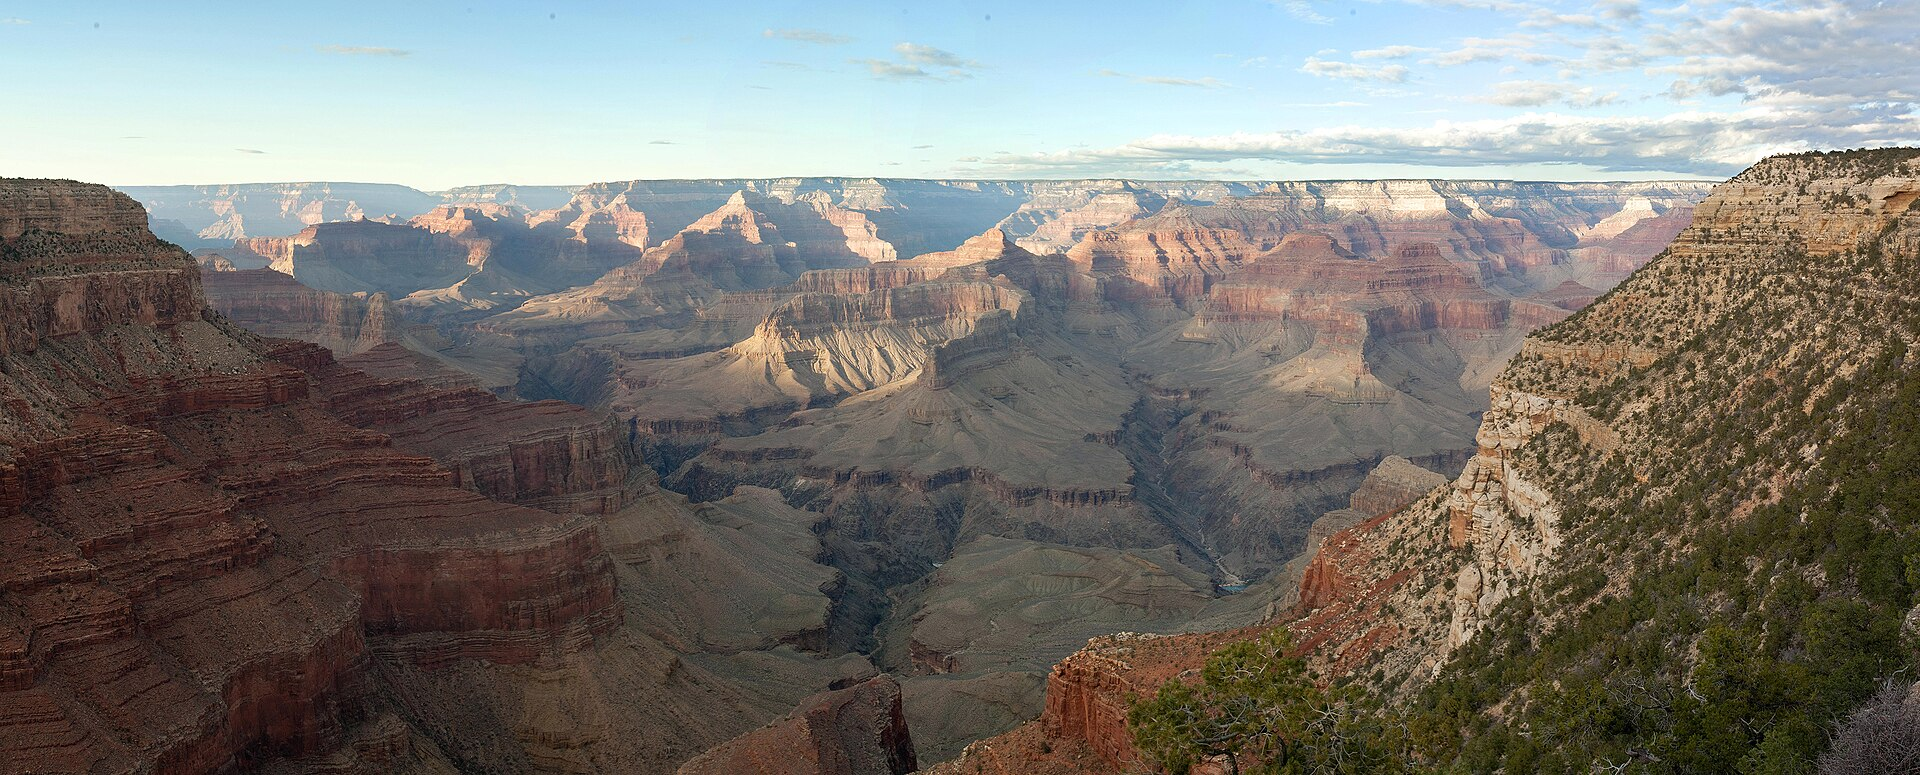
\includegraphics[width=\linewidth]{images/book1/g7-grand-canyon.jpg}

{\small ग्रैंड कैन्यन, उसके दक्षिणी किनारे पर हर्मिट्स रेस्ट से: किनारे से तली तक
\omterm{def:g3:stones-pebbles-sand:rock}{चट्टान} की परत-दर-परत। राष्ट्रीय उद्यान सेवा की फ़ोटो, क्रिस्टन कैल्डन द्वारा
(सार्वजनिक डोमेन, विकिमीडिया कॉमन्स के ज़रिए)।}
% ledger: commons:grand-canyon
\label{fig:g7:sediments-and-fossils:canyon}
\end{omfigure}

ढीली \omterm{def:g3:stones-pebbles-sand:sand}{रेत} और \omterm{def:g3:stones-pebbles-sand:sand}{कीचड़} का ढेर ठोस \omterm{def:g3:stones-pebbles-sand:rock}{चट्टान} कैसे बन जाता है? एक सीपी इतने लंबे समय तक कैसे
बची रह सकती है कि वह किसी खड़ी \omterm{def:g3:stones-pebbles-sand:rock}{चट्टान} के अंदर पहुँच जाए? और परतें और \omterm{def:g7:sediments-and-fossils:fossil}{जीवाश्म}
हमें बहुत पहले की जगहों के बारे में क्या बताते हैं?

\begin{recall}
सतह पर \omterm{def:g3:stones-pebbles-sand:rock}{चट्टानें} धीरे-धीरे टुकड़ों में टूटती हैं (\emph{\omterm{def:g5:water-shapes-the-land:weathering}{अपक्षय}}); पानी, हवा और बर्फ़
टुकड़ों को बहा ले जाते हैं (\emph{\omterm{def:g5:water-shapes-the-land:erosion}{अपरदन}}) और उन्हें वहाँ बिछा देते हैं जहाँ वे
धीमे होकर रुक जाते हैं (\emph{\omterm{def:g5:water-shapes-the-land:deposition}{निक्षेपण}}): सबसे भारी पहले, महीन \omterm{def:g3:stones-pebbles-sand:sand}{कीचड़} केवल वहाँ
जहाँ पानी लगभग स्थिर है (\cref{ch:g5:water-shapes-the-land})। \emph{\omterm{def:g6:rocks-and-minerals:rock-families}{अवसादी
चट्टान}} सतह पर \omterm{def:g3:stones-pebbles-sand:sand}{रेत} और \omterm{def:g3:stones-pebbles-sand:sand}{कीचड़} के कणों से, या सीपियों से, बनती है जो परतों में बिछकर
सख़्त हो गए हों: बलुआ पत्थर, शेल, चूना पत्थर। \omterm{def:g6:rocks-and-minerals:rock-cycle}{शैल चक्र} हर परिवार की \omterm{def:g3:stones-pebbles-sand:rock}{चट्टानों} को,
धीरे-धीरे, दूसरों में बदलता है
(\cref{ch:g6:rocks-and-minerals})।
\end{recall}

\section{अवसाद परतों में बैठते हैं}

जहाँ भी पानी, हवा या बर्फ़ अपने साथ लाई चीज़ें गिरा देते हैं, वहाँ एक ढीला जमाव
बनता जाता है: \omterm{def:g1:landscapes-around-us:water}{नदी} के तल पर \omterm{def:g3:stones-pebbles-sand:pebble}{बजरी} और \omterm{def:g3:stones-pebbles-sand:sand}{रेत}, \omterm{def:g1:landscapes-around-us:water}{झील} की तली पर \omterm{def:g3:stones-pebbles-sand:sand}{कीचड़}, \omterm{def:g2:water-on-earth:ocean}{समुद्र} \omterm{def:g1:landscapes-around-us:water}{तट} पर या
टीले में \omterm{def:g3:stones-pebbles-sand:sand}{रेत}, \omterm{def:g2:water-on-earth:ocean}{समुद्र} की तली पर सीपियाँ।

\begin{definition}[अवसाद]\label{def:g7:sediments-and-fossils:sediment}
\emph{अवसाद}\index{अवसाद} पानी, हवा या बर्फ़ द्वारा बिछाया गया ढीला पदार्थ है:
\omterm{def:g3:stones-pebbles-sand:pebble}{बजरी}, \omterm{def:g3:stones-pebbles-sand:sand}{रेत}, \omterm{def:g3:stones-pebbles-sand:sand}{कीचड़}, या जीवों की सीपियाँ और कंकाल। यह \omterm{def:g1:landscapes-around-us:water}{नदियों}, \omterm{def:g1:landscapes-around-us:water}{झीलों} और \omterm{def:g2:water-on-earth:ocean}{समुद्रों} की
तली पर जमा होता है, और ज़मीन पर वहाँ जहाँ हवा या बर्फ़ उसे गिरा
देती है।
\end{definition}

\omterm{def:g7:sediments-and-fossils:sediment}{अवसाद} एक ख़ास क्रम में बैठते हैं। जब \omterm{def:g3:stones-pebbles-sand:sand}{कीचड़} भरा पानी धीमा होता है, तो सबसे बड़े
और भारी कण पहले डूबते हैं और सबसे छोटे और हल्के सबसे आख़िर में। हर बार जब पानी
बदलता है --- एक \omterm{def:g5:water-shapes-the-land:flood}{बाढ़} जो \omterm{def:g3:stones-pebbles-sand:sand}{रेत} लाती है, फिर शांत हफ़्ते जब केवल महीन \omterm{def:g3:stones-pebbles-sand:sand}{कीचड़} तली तक
पहुँचता है --- तो बैठने वाले कण भी बदल जाते हैं, और एक नई परत शुरू होती है।
धीरे-धीरे \omterm{def:g1:landscapes-around-us:water}{झील} या \omterm{def:g2:water-on-earth:ocean}{समुद्र} की तली परतों के एक ढेर से ढक जाती है, जिसमें सबसे पुरानी
परत ढेर के सबसे
नीचे होती है।
% ledger: usgs:strata, usgs:sediments-to-rock

\begin{omfigure}
\begin{tikzpicture}[font=\small, x=1cm, y=1cm]
  % land and river
  \fill[omLithAlluv] (0,3.0) -- (2.0,2.45) -- (2.0,0) -- (0,0) -- cycle;
  \fill[blue!35] (0,3.05) -- (2.0,2.5) -- (2.0,2.4) -- (0,2.95) -- cycle;
  % lake water
  \fill[omSea!45] (2.0,2.5) -- (12.4,2.5) -- (12.4,1.12) -- (3.0,1.2) -- cycle;
  \draw[blue!50!black, line width=0.6pt] (2.0,2.5) -- (12.4,2.5);
  % layers on the bottom: thick near the mouth, thinner far out
  \foreach \k/\c in {0/omLithSand, 1/omLithShale, 2/omLithSand, 3/omLithShale} {
    \pgfmathsetmacro{\yb}{0.2+0.25*\k}
    \pgfmathsetmacro{\yt}{0.2+0.25*(\k+1)}
    \fill[\c] (3.0,\yb) -- (12.4,\yb) -- (12.4,\yt-0.08) -- (3.0,\yt) -- cycle;
  }
  \draw[black!60, line width=0.3pt] (3.0,1.2) -- (12.4,1.12);
  \fill[omLithAlluv!80!black] (2.0,0) rectangle (12.4,0.2);
  \fill[omLithAlluv] (2.0,0.2) -- (3.0,0.2) -- (3.0,1.2) -- (2.0,2.45) -- cycle;
  % settling grains: big ones near the mouth, fine ones far out
  \foreach \x/\y in {3.3/2.1, 3.6/1.75, 3.9/2.25, 4.2/1.55, 3.5/1.35, 4.5/2.0} {
    \fill[brown!70!black] (\x,\y) circle (0.07);
    \draw[-{Stealth[length=1.3mm]}, black!60] (\x,\y-0.1) -- (\x,\y-0.32);
  }
  \foreach \x/\y in {6.5/2.2, 7.4/1.8, 8.3/2.15, 9.1/1.6, 9.9/2.05, 10.8/1.75, 11.6/2.1, 7.9/1.35, 10.4/1.3} {
    \fill[brown!50!black] (\x,\y) circle (0.025);
    \draw[-{Stealth[length=1mm]}, black!40] (\x,\y-0.05) -- (\x,\y-0.2);
  }
  \node[anchor=south, align=center] at (1.0,3.1) {बाढ़ वाली नदी\\[-2pt]रेत और कीचड़ लाती है};
  \node[anchor=south, align=center] at (4.1,2.55) {रेत पहले, मुहाने\\[-2pt]के पास बैठती है};
  \node[anchor=south, align=center] at (9.2,2.55) {महीन कीचड़ धीरे-धीरे, दूर,\\[-2pt]शांत पानी में बैठता है};
  \draw[decorate, decoration={brace, amplitude=4pt}] (12.55,1.15) -- (12.55,0.2)
    node[midway, anchor=west, xshift=4pt, align=left, font=\footnotesize] {तली पर\\[-2pt]परतें: रेत,\\[-2pt]कीचड़, रेत, कीचड़};
\end{tikzpicture}

{\small एक \omterm{def:g1:landscapes-around-us:water}{झील} में बैठता \omterm{def:g7:sediments-and-fossils:sediment}{अवसाद} (एक चित्र, पैमाने पर नहीं)। हर \omterm{def:g5:water-shapes-the-land:flood}{बाढ़} के बाद \omterm{def:g3:stones-pebbles-sand:sand}{रेत} की
एक परत बैठती है, फिर उसके बाद के शांत हफ़्तों में महीन \omterm{def:g3:stones-pebbles-sand:sand}{कीचड़}: तली पर परत-दर-परत
जमा होती जाती है।}
% ledger: usgs:strata
\label{fig:g7:sediments-and-fossils:lake}
\end{omfigure}

\begin{definition}[अवसादी परत]\label{def:g7:sediments-and-fossils:layer}
\emph{अवसादी परत}\index{अवसादी परत}, या \emph{स्तर}\index{स्तर} (बहुवचन भी
\emph{स्तर}), \omterm{def:g7:sediments-and-fossils:sediment}{अवसाद} की, या उससे बनी \omterm{def:g3:stones-pebbles-sand:rock}{चट्टान} की, एक चादर है जो एक ही समय में बिछी
हो। उसका एक आधार और एक ऊपरी सतह होती है, और वह अपने ऊपर और नीचे की परतों से
अपने कणों के आकार में या अपनी बनावट में
अलग होती है।
\end{definition}

\omterm{def:g7:sediments-and-fossils:sediment}{अवसाद} पानी या हवा से बैठते हैं, इसलिए वे समतल बिछते हैं, मेज़ पर रखी किसी किताब
के पन्नों की तरह। जब परतें झुकी या मुड़ी हुई मिलती हैं, तो उनके बनने के बाद किसी
चीज़ ने उन्हें हिलाया है। परतें होना \omterm{def:g6:rocks-and-minerals:rock-families}{अवसादी चट्टान} की सबसे साफ़ पहचान है: तुमने
इसे ग्रैंड कैन्यन की दीवारों में देखा।
% ledger: usgs:strata, nps:grca-kaibab

\begin{inthelab}[मर्तबान में परतें (कक्षा में, अध्यापक के साथ)]
एक लंबे काँच के मर्तबान में एक मुट्ठी \omterm{def:g3:stones-pebbles-sand:pebble}{बजरी}, दो मुट्ठी \omterm{def:g3:stones-pebbles-sand:sand}{रेत} और कुछ चम्मच मिट्टी
डालो; उसे पानी से भरो, कसकर बंद करो और हिलाओ। उसे रख दो और कुछ मिनट देखो: \omterm{def:g3:stones-pebbles-sand:pebble}{बजरी}
तुरंत तली तक पहुँच जाती है, \omterm{def:g3:stones-pebbles-sand:sand}{रेत} थोड़ी देर बाद, और महीन \omterm{def:g3:stones-pebbles-sand:sand}{कीचड़} पानी को घंटों तक
गदला रखता है। अगले दिन थोड़ी और मिट्टी और \omterm{def:g3:stones-pebbles-sand:sand}{रेत} डालो, धीरे से हिलाओ, और उसे फिर
बैठने दो। तुम कितनी परतें गिन सकते हो? हर परत के नीचे कौन-से कण
हैं?
\end{inthelab}

\section{अवसाद से चट्टान तक}

कोई परत लंबे समय तक सबसे ऊपर नहीं रहती। उसके ऊपर दूसरी परतें बैठती हैं, फिर और,
और वह गहरे से गहरे दबती जाती है। ऊपर की परतों के भार से कण एक-दूसरे के और पास
दब जाते हैं और उनके बीच का पानी निचुड़ जाता है। ढेर में से रिसता पानी कणों के बीच
\omterm{def:g6:rocks-and-minerals:mineral}{खनिज} छोड़ जाता है, एक प्राकृतिक सीमेंट जो उन्हें आपस में चिपका देता है। लंबे समय
में, और परतें जमा होने और धीमे रासायनिक बदलावों से, ढेर के नीचे का ढीला \omterm{def:g7:sediments-and-fossils:sediment}{अवसाद}
\omterm{def:g3:stones-pebbles-sand:rock}{चट्टान} बन जाता है।
% ledger: usgs:sediments-to-rock, usgs:sedimentary

हर तरह का \omterm{def:g7:sediments-and-fossils:sediment}{अवसाद} अपनी \omterm{def:g3:stones-pebbles-sand:rock}{चट्टान} बनाता है।

\begin{center}
\small
\begin{tabular}{|l|l|}
\hline
\textbf{\omterm{def:g7:sediments-and-fossils:sediment}{अवसाद}} & \textbf{वह \omterm{def:g3:stones-pebbles-sand:rock}{चट्टान} जो वह बनता है} \\
\hline
\omterm{def:g3:stones-pebbles-sand:pebble}{बजरी} और \omterm{def:g3:stones-pebbles-sand:pebble}{कंकड़} & कांग्लोमरेट \\
\omterm{def:g3:stones-pebbles-sand:sand}{रेत} & बलुआ पत्थर \\
\omterm{def:g3:stones-pebbles-sand:sand}{कीचड़} & पंकाश्म, या शेल जब वह पतली चादरों में टूटता है \\
सीपियाँ और कंकाल & चूना पत्थर \\
दलदल में दबे पौधों के अवशेष & कोयला \\
\hline
\end{tabular}
\end{center}
% ledger: usgs:sediments-to-rock, usgs:sedimentary, usgs:coal-origin

\begin{omfigure}
\begin{tikzpicture}[font=\small, x=1cm, y=1cm]
  \pgfmathsetseed{11}
  \foreach \p/\gap/\title in {0/0.40/{ढीला अवसाद}, 1/0.31/{दबा और भिंचा:\\[-2pt]पानी बाहर निकला}, 2/0.31/{सीमेंट से जुड़ा: एक चट्टान}} {
    \begin{scope}[xshift=\p*4.6cm]
      \ifnum\p=2 \fill[black!25] (0,0) rectangle (3.4,3.0);
      \else \fill[omSea!45] (0,0) rectangle (3.4,3.0); \fi
      \foreach \i in {0,...,7} {
        \foreach \j in {0,...,6} {
          \pgfmathsetmacro{\gx}{0.25 + \i*\gap*1.05 + 0.05*rand}
          \pgfmathsetmacro{\gy}{0.25 + \j*\gap + 0.05*rand}
          \pgfmathsetmacro{\gr}{0.13 + 0.03*rand}
          \ifdim\gx pt<3.25pt \ifdim\gy pt<2.85pt
            \fill[omLithSand!80!brown, draw=brown!60!black, line width=0.3pt] (\gx,\gy) circle (\gr);
          \fi\fi
        }
      }
      \draw[black!70, line width=0.6pt] (0,0) rectangle (3.4,3.0);
      \node[anchor=north, align=center] at (1.7,-0.1) {\title};
    \end{scope}
  }
  \draw[-{Stealth[length=2.5mm]}, line width=1pt] (3.6,1.5) -- (4.4,1.5);
  \draw[-{Stealth[length=2.5mm]}, line width=1pt] (8.2,1.5) -- (9.0,1.5);
  \foreach \x in {5.3,6.3,7.3} \draw[-{Stealth[length=2mm]}, line width=0.8pt] (\x,3.7) -- (\x,3.1);
  \node[anchor=south] at (6.3,3.7) {ऊपर की परतों का भार};
  \node[anchor=south, font=\footnotesize, align=center] at (10.9,3.05) {धूसर: प्राकृतिक सीमेंट};
\end{tikzpicture}

{\small \omterm{def:g3:stones-pebbles-sand:sand}{रेत} से बलुआ पत्थर तक (कणों का एक चित्र, बहुत बड़ा करके)। बाएँ: ढीले कण,
उनके बीच पानी। बीच में: नई परतों के नीचे दबकर कण एक-दूसरे से भिंच जाते हैं।
दाएँ: पानी के छोड़े \omterm{def:g6:rocks-and-minerals:mineral}{खनिज} कणों को आपस में चिपका देते
हैं।}
% ledger: usgs:sediments-to-rock, usgs:sedimentary
\label{fig:g7:sediments-and-fossils:to-rock}
\end{omfigure}

पृथ्वी की सतह पर तुम जो \omterm{def:g3:stones-pebbles-sand:rock}{चट्टानें} देख सकते हो, उनमें से ज़्यादातर अवसादी हैं। वे
परतों का जो ढेर बनाती हैं, वह उस जगह के इतिहास की किताब है: हर परत एक पन्ना है,
और सबसे पुराने पन्ने सबसे नीचे हैं।
% ledger: usgs:sediments-to-rock

\section{जीवाश्म कैसे बनता है}

\begin{definition}[जीवाश्म]\label{def:g7:sediments-and-fossils:fossil}
\emph{जीवाश्म}\index{जीवाश्म} बहुत पहले के किसी जीव के अवशेष, या उसका निशान,
है जो \omterm{def:g3:stones-pebbles-sand:rock}{चट्टान} में सुरक्षित रहा हो। कुछ जीवाश्म शरीर के सख़्त हिस्से हैं --- सीपी,
हड्डी, दाँत, लकड़ी --- जो पत्थर बन गए। दूसरे केवल एक आकार बचाते हैं:
\emph{साँचा}\index{साँचा} \omterm{def:g3:stones-pebbles-sand:rock}{चट्टान} में बचा खोखला छाप है जहाँ कोई सीपी या हड्डी
घुल गई हो; \emph{ढलाई}\index{ढलाई} वह प्रतिरूप है जो तब बनता है जब कोई साँचा
नए \omterm{def:g6:rocks-and-minerals:mineral}{खनिज} पदार्थ या \omterm{def:g7:sediments-and-fossils:sediment}{अवसाद} से भर जाता है। \emph{चिह्न जीवाश्म}\index{चिह्न जीवाश्म}
किसी जानवर के किए काम का संकेत है --- पैरों का निशान, बिल, घिसटने की लकीर --- न
कि उसके शरीर का कोई
हिस्सा।
\end{definition}

\omterm{def:g7:sediments-and-fossils:fossil}{जीवाश्म} अपनी ज़िंदगी \omterm{def:g2:water-on-earth:ocean}{समुद्र} या \omterm{def:g1:landscapes-around-us:water}{झील} की तली पर एक मरे हुए जानवर या पौधे के रूप में
शुरू करता है। अगर वह खुला पड़ा रहे, तो जीवाणु उसे तोड़ देते हैं और पानी जो बचा
है उसे धीरे-धीरे घोल देता है। उसके बचने की संभावना तभी है जब वह जल्दी दब जाए,
अपने ऊपर बैठने वाले \omterm{def:g7:sediments-and-fossils:sediment}{अवसाद} के नीचे जो उसे बंद कर दे। फिर, जैसे-जैसे \omterm{def:g7:sediments-and-fossils:sediment}{अवसाद} \omterm{def:g3:stones-pebbles-sand:rock}{चट्टान}
बनता है, परतों में से रिसता पानी \omterm{def:g6:rocks-and-minerals:mineral}{खनिज} लाता है जो सीपी या हड्डी के हर नन्हे छेद को
भर देते हैं: वह पत्थर बन जाती है। बहुत बाद में, ऊपर की परतें घिसकर हट सकती हैं,
और \omterm{def:g7:sediments-and-fossils:fossil}{जीवाश्म} सतह पर दिखने
लगता है।
% ledger: ucmp:fossil-conditions, ucmp:fossil-kinds, usgs:sediments-to-rock

\begin{omfigure}
\begin{tikzpicture}[font=\small, x=0.86cm, y=0.86cm,
    shell/.pic={
      \fill[#1] (0,0) circle (0.42);
      \draw[brown!40!black, line width=0.5pt] plot[domain=0:12.5, samples=90, smooth]
        ({0.032*\x*cos(\x r)}, {0.032*\x*sin(\x r)});
      \draw[brown!40!black, line width=0.5pt] (0,0) circle (0.42);
    }]
  % 1: death on the sea floor
  \begin{scope}[xshift=0cm]
    \fill[omSea!45] (0,1.2) rectangle (3.3,3.6);
    \fill[omLithShale] (0,0) rectangle (3.3,1.2);
    \pic at (1.65,1.62) {shell=omLithSand!60!white};
    \node[anchor=north, align=center] at (1.65,-0.1) {1. वह समुद्र की\\[-2pt]तली पर मरता है};
  \end{scope}
  % 2: quick burial
  \begin{scope}[xshift=3.75cm]
    \fill[omSea!45] (0,2.1) rectangle (3.3,3.6);
    \fill[omLithShale] (0,0) rectangle (3.3,1.2);
    \fill[omLithShale!70!white] (0,1.2) rectangle (3.3,2.1);
    \pic at (1.65,1.62) {shell=omLithSand!60!white};
    \foreach \x in {0.5,1.2,2.1,2.8} \fill[brown!50!black] (\x,2.4) circle (0.03);
    \node[anchor=north, align=center] at (1.65,-0.1) {2. कीचड़ उसे जल्दी\\[-2pt]ढक लेता है};
  \end{scope}
  % 3: buried deep, turned to stone
  \begin{scope}[xshift=7.5cm]
    \fill[omLithShale!80!black] (0,0) rectangle (3.3,1.2);
    \fill[omLithShale!85!black] (0,1.2) rectangle (3.3,2.1);
    \fill[omLithSand] (0,2.1) rectangle (3.3,2.9);
    \fill[omLithLime] (0,2.9) rectangle (3.3,3.6);
    \pic at (1.65,1.62) {shell=black!35};
    \node[anchor=north, align=center] at (1.65,-0.1) {3. गहरे दबकर वह\\[-2pt]पत्थर बन जाता है};
  \end{scope}
  % 4: uncovered by erosion
  \begin{scope}[xshift=11.25cm]
    \fill[white] (0,0) rectangle (3.3,3.6);
    \fill[omLithShale!80!black] (0,0) -- (3.3,0) -- (3.3,2.6) -- (2.4,2.3) -- (1.8,1.95) -- (1.2,1.7) -- (0,1.5) -- cycle;
    \draw[black!35, line width=0.4pt] (0,1.2) -- (3.3,1.2);
    \draw[black!60, line width=0.4pt] (0,1.5) -- (1.2,1.7) -- (1.8,1.95) -- (2.4,2.3) -- (3.3,2.6);
    \pic at (1.65,1.84) {shell=black!35};
    \node[anchor=north, align=center] at (1.65,-0.1) {4. अपरदन उसे\\[-2pt]सतह पर ले आता है};
  \end{scope}
  \foreach \p in {0,1,2,3} {
    \begin{scope}[xshift=\p*3.75cm]
      \draw[black!70, line width=0.5pt] (0,0) rectangle (3.3,3.6);
    \end{scope}
  }
\end{tikzpicture}

{\small \omterm{def:g7:sediments-and-fossils:fossil}{जीवाश्म} कैसे बनता है (एक चित्र, पैमाने पर नहीं): एक सीपी \omterm{def:g3:stones-pebbles-sand:sand}{कीचड़} के नीचे
जल्दी दब जाती है; नई परतों के नीचे और गहरे दबकर वह पत्थर बन जाती है; बहुत बाद
में \omterm{def:g5:water-shapes-the-land:erosion}{अपरदन} ऊपर की परतों को घिस देता है और \omterm{def:g7:sediments-and-fossils:fossil}{जीवाश्म} सतह पर दिखने
लगता है।}
% ledger: ucmp:fossil-conditions, ucmp:fossil-kinds
\label{fig:g7:sediments-and-fossils:steps}
\end{omfigure}

ज़्यादातर जीव कोई \omterm{def:g7:sediments-and-fossils:fossil}{जीवाश्म} नहीं छोड़ते। नरम शरीर दबने से पहले ही सड़ जाते हैं;
सीपियाँ और हड्डियाँ भी लंबे समय तक खुली पड़ी रहें तो टूट जाती हैं या घुल जाती
हैं। \omterm{def:g7:sediments-and-fossils:fossil}{जीवाश्म} बनने के लिए सबसे अच्छी जगह किसी शांत \omterm{def:g2:water-on-earth:ocean}{समुद्र} या \omterm{def:g1:landscapes-around-us:water}{झील} की तली है, जहाँ
महीन \omterm{def:g3:stones-pebbles-sand:sand}{कीचड़} अवशेषों पर बैठकर उन्हें बचाता है। इसीलिए \omterm{def:g3:stones-pebbles-sand:rock}{चट्टानों} में मिलने वाले
\omterm{def:g7:sediments-and-fossils:fossil}{जीवाश्म} ज़्यादातर सीपियाँ हैं, और सूक्ष्म पौधों और जानवरों की नन्ही सीपियाँ और
अवशेष; डायनासोर, सबसे प्रसिद्ध \omterm{def:g7:sediments-and-fossils:fossil}{जीवाश्म}, उनका केवल एक बहुत छोटा
हिस्सा हैं।
% ledger: ucmp:fossil-conditions, usgs:fossil-record-shells

\begin{omfigure}
\begin{minipage}[t]{0.49\linewidth}\centering
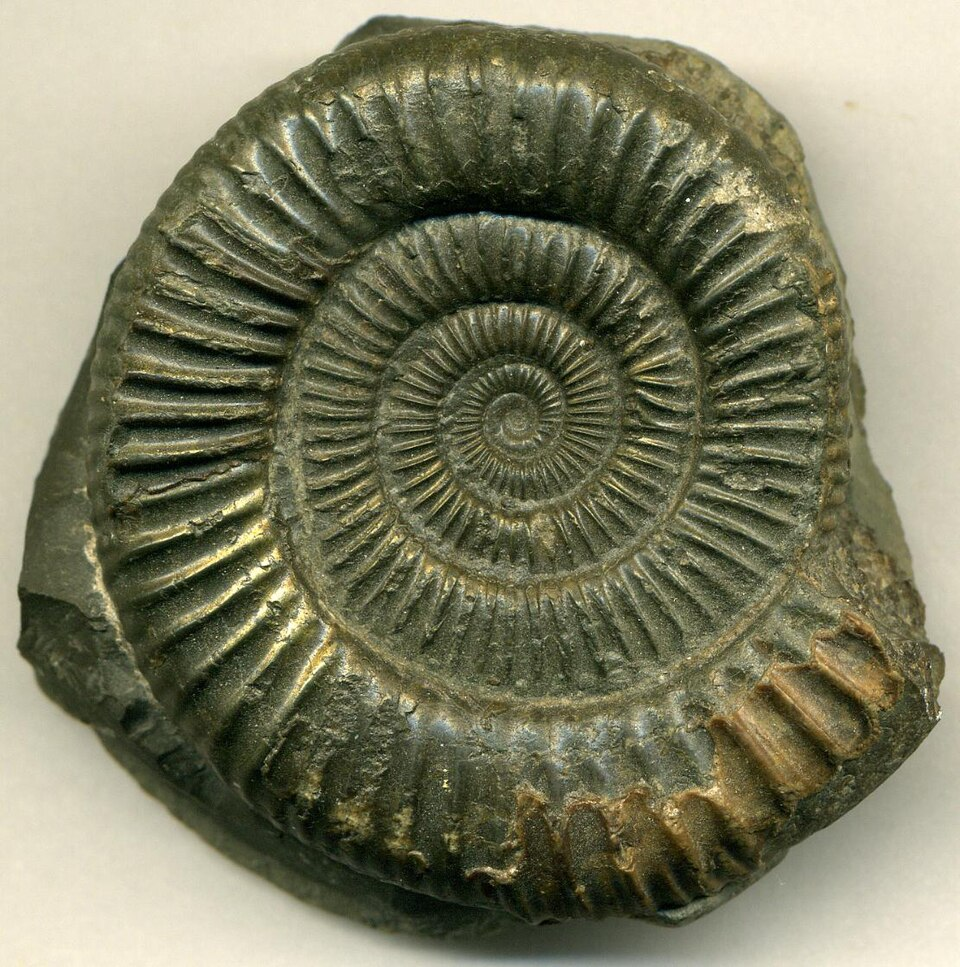
\includegraphics[height=4.6cm]{images/book1/g7-ammonite.jpg}

{\small एक अमोनाइट, कुंडलित सीपी वाला एक विलुप्त जानवर, स्क्विड और ऑक्टोपस का
एक संबंधी, \qty{5.7}{cm} चौड़ा, यॉर्कशायर (इंग्लैंड) के \omterm{def:g1:landscapes-around-us:water}{तट}
से।}
\end{minipage}\hfill
\begin{minipage}[t]{0.49\linewidth}\centering
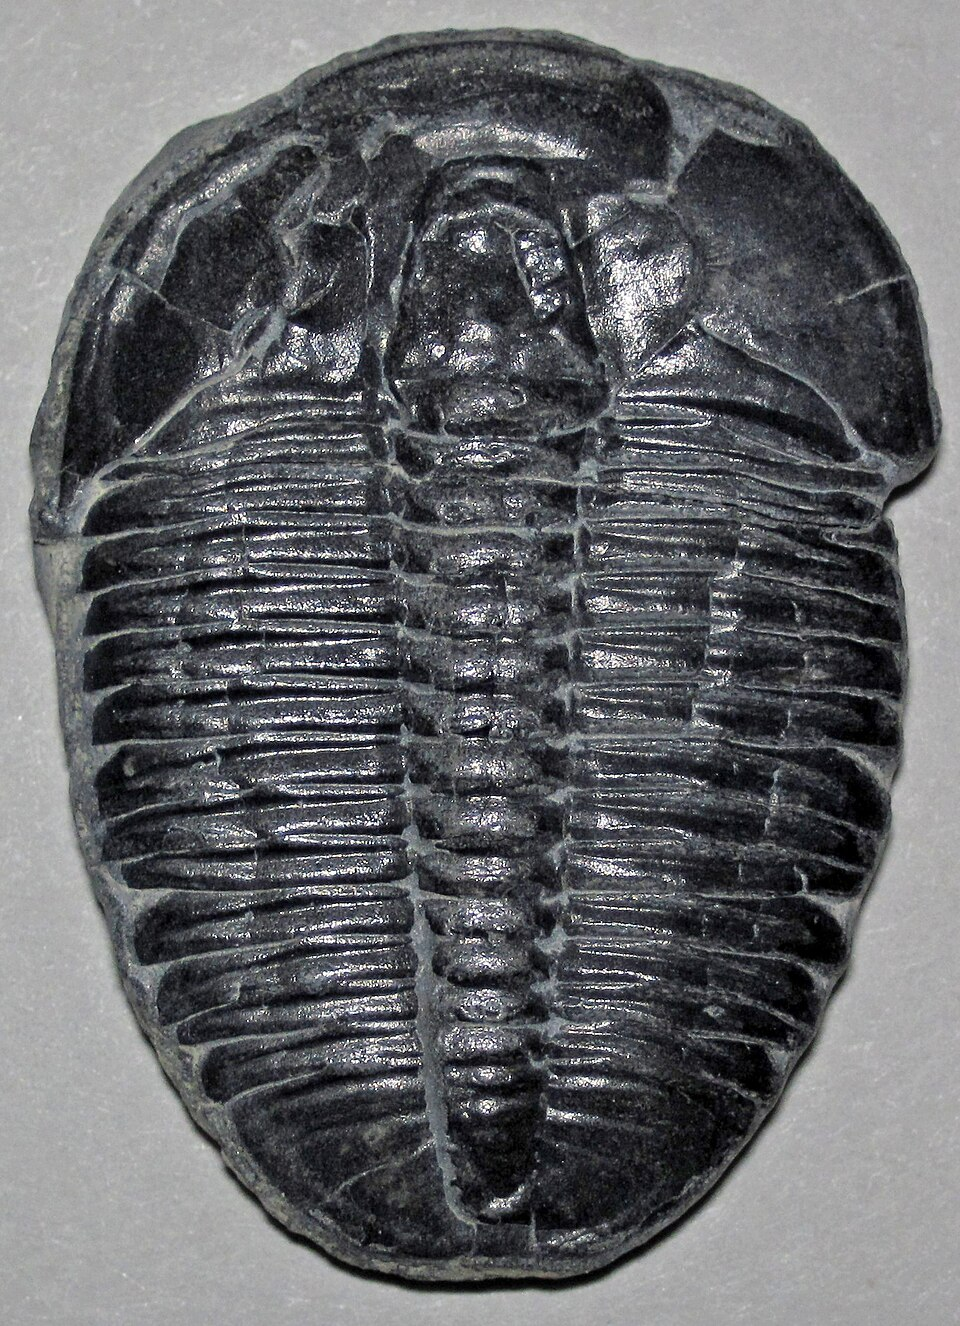
\includegraphics[height=4.6cm]{images/book1/g7-trilobite.jpg}

{\small एक ट्राइलोबाइट, \omterm{def:g2:water-on-earth:ocean}{समुद्र} का एक विलुप्त जानवर जिसके शरीर में तीन खंड हैं,
लगभग \qty{2.6}{cm} चौड़ा, यूटा (संयुक्त राज्य अमेरिका) से।}
\end{minipage}\par\medskip

{\small सख़्त खोल वाले जानवरों के दो \omterm{def:g7:sediments-and-fossils:fossil}{जीवाश्म}। फ़ोटो: जेम्स
सेंट~जॉन (CC BY 2.0, विकिमीडिया कॉमन्स के ज़रिए)।}
% ledger: commons:ammonite, commons:trilobite, nps:ammonoid, nps:trilobite
\label{fig:g7:sediments-and-fossils:ammonite-trilobite}
\end{omfigure}

कभी-कभी सीपी ख़ुद नहीं बचती। \omterm{def:g3:stones-pebbles-sand:sand}{रेत} में दबी होने पर वह कणों के बीच से रिसते पानी से
धीरे-धीरे घुल जाती है, और केवल एक खोखली जगह बचती है, जिसकी दीवारों पर सीपी का
आकार छपा होता है: एक \omterm{def:g7:sediments-and-fossils:fossil}{साँचा}। अगर बाद में \omterm{def:g6:rocks-and-minerals:mineral}{खनिज} उस खोखली जगह में बैठकर उसे भर दें, तो
वे सीपी का एक प्रतिरूप बनाते हैं: एक
\omterm{def:g7:sediments-and-fossils:fossil}{ढलाई}।
% ledger: ucmp:casts-molds

\begin{omfigure}
\begin{tikzpicture}[font=\small, x=1cm, y=1cm,
    clam/.style={line width=0.5pt}]
  \foreach \p/\fillc/\title in {0/{omLithSand!50!white}/{रेत में दबी\\[-2pt]एक सीपी}, 1/{white}/{सीपी घुल गई:\\[-2pt]एक साँचा}, 2/{black!40}/{खनिज साँचे को भरते हैं:\\[-2pt]एक ढलाई}} {
    \begin{scope}[xshift=\p*4.9cm]
      \fill[omLithSand] (0,0) rectangle (4.2,2.6);
      \foreach \i in {0,...,40} {
        \pgfmathsetmacro{\gx}{0.1+mod(\i*0.53,4.0)}
        \pgfmathsetmacro{\gy}{0.1+mod(\i*0.37,2.4)}
        \fill[brown!60!black] (\gx,\gy) circle (0.025);
      }
      \fill[\fillc, draw=brown!40!black, clam] (0.9,0.9) arc[start angle=180, end angle=0, x radius=1.2, y radius=0.95] -- cycle;
      \ifnum\p=1
        \foreach \a in {25,45,...,155} \draw[brown!50!black, line width=0.4pt] (2.1,0.9) -- ++(\a:0.93 and 0.75);
      \else
        \foreach \a in {25,45,...,155} \draw[brown!40!black, line width=0.4pt] (2.1,0.9) -- ++(\a:1.05 and 0.85);
      \fi
      \draw[black!70, line width=0.5pt] (0,0) rectangle (4.2,2.6);
      \node[anchor=north, align=center] at (2.1,-0.1) {\title};
    \end{scope}
  }
  \draw[-{Stealth[length=2.5mm]}, line width=1pt] (4.3,1.3) -- (4.8,1.3);
  \draw[-{Stealth[length=2.5mm]}, line width=1pt] (9.2,1.3) -- (9.7,1.3);
\end{tikzpicture}

{\small एक \omterm{def:g7:sediments-and-fossils:fossil}{साँचा} और एक \omterm{def:g7:sediments-and-fossils:fossil}{ढलाई} (\omterm{def:g3:stones-pebbles-sand:rock}{चट्टान} को काटकर बना एक चित्र)। \omterm{def:g7:sediments-and-fossils:fossil}{साँचा} खोखली जगह है,
जिसकी दीवार पर सीपी की धारियाँ छपी हैं; \omterm{def:g7:sediments-and-fossils:fossil}{ढलाई} सीपी का पत्थर का प्रतिरूप है, जो उन
\omterm{def:g6:rocks-and-minerals:mineral}{खनिजों} से बना है जिन्होंने उसे भरा।}
% ledger: ucmp:casts-molds
\label{fig:g7:sediments-and-fossils:mould-cast}
\end{omfigure}

जानवर अपने किए कामों के भी \omterm{def:g7:sediments-and-fossils:fossil}{जीवाश्म} छोड़ते हैं। \omterm{def:g1:landscapes-around-us:water}{नदी} के किनारे या \omterm{def:g1:landscapes-around-us:water}{तट} की नरम, गीली
\omterm{def:g3:stones-pebbles-sand:sand}{कीचड़} पर चलता कोई जानवर पैरों के निशान छोड़ता है। ज़्यादातर निशान अगली लहर या अगली
\omterm{def:g5:water-shapes-the-land:flood}{बाढ़} में धुल जाते हैं। पर अगर मिटने से पहले \omterm{def:g3:stones-pebbles-sand:sand}{रेत} उन्हें ढक ले, तो निशान भर जाता
है, \omterm{def:g3:stones-pebbles-sand:sand}{रेत} बाद में बलुआ पत्थर बन जाती है, और जब \omterm{def:g3:stones-pebbles-sand:rock}{चट्टान} परत के साथ-साथ फटती है, तो
वह पैर का निशान और, दूसरी ओर, उसकी \omterm{def:g7:sediments-and-fossils:fossil}{ढलाई}
दिखाती है।
% ledger: ucmp:footprints

\begin{omfigure}
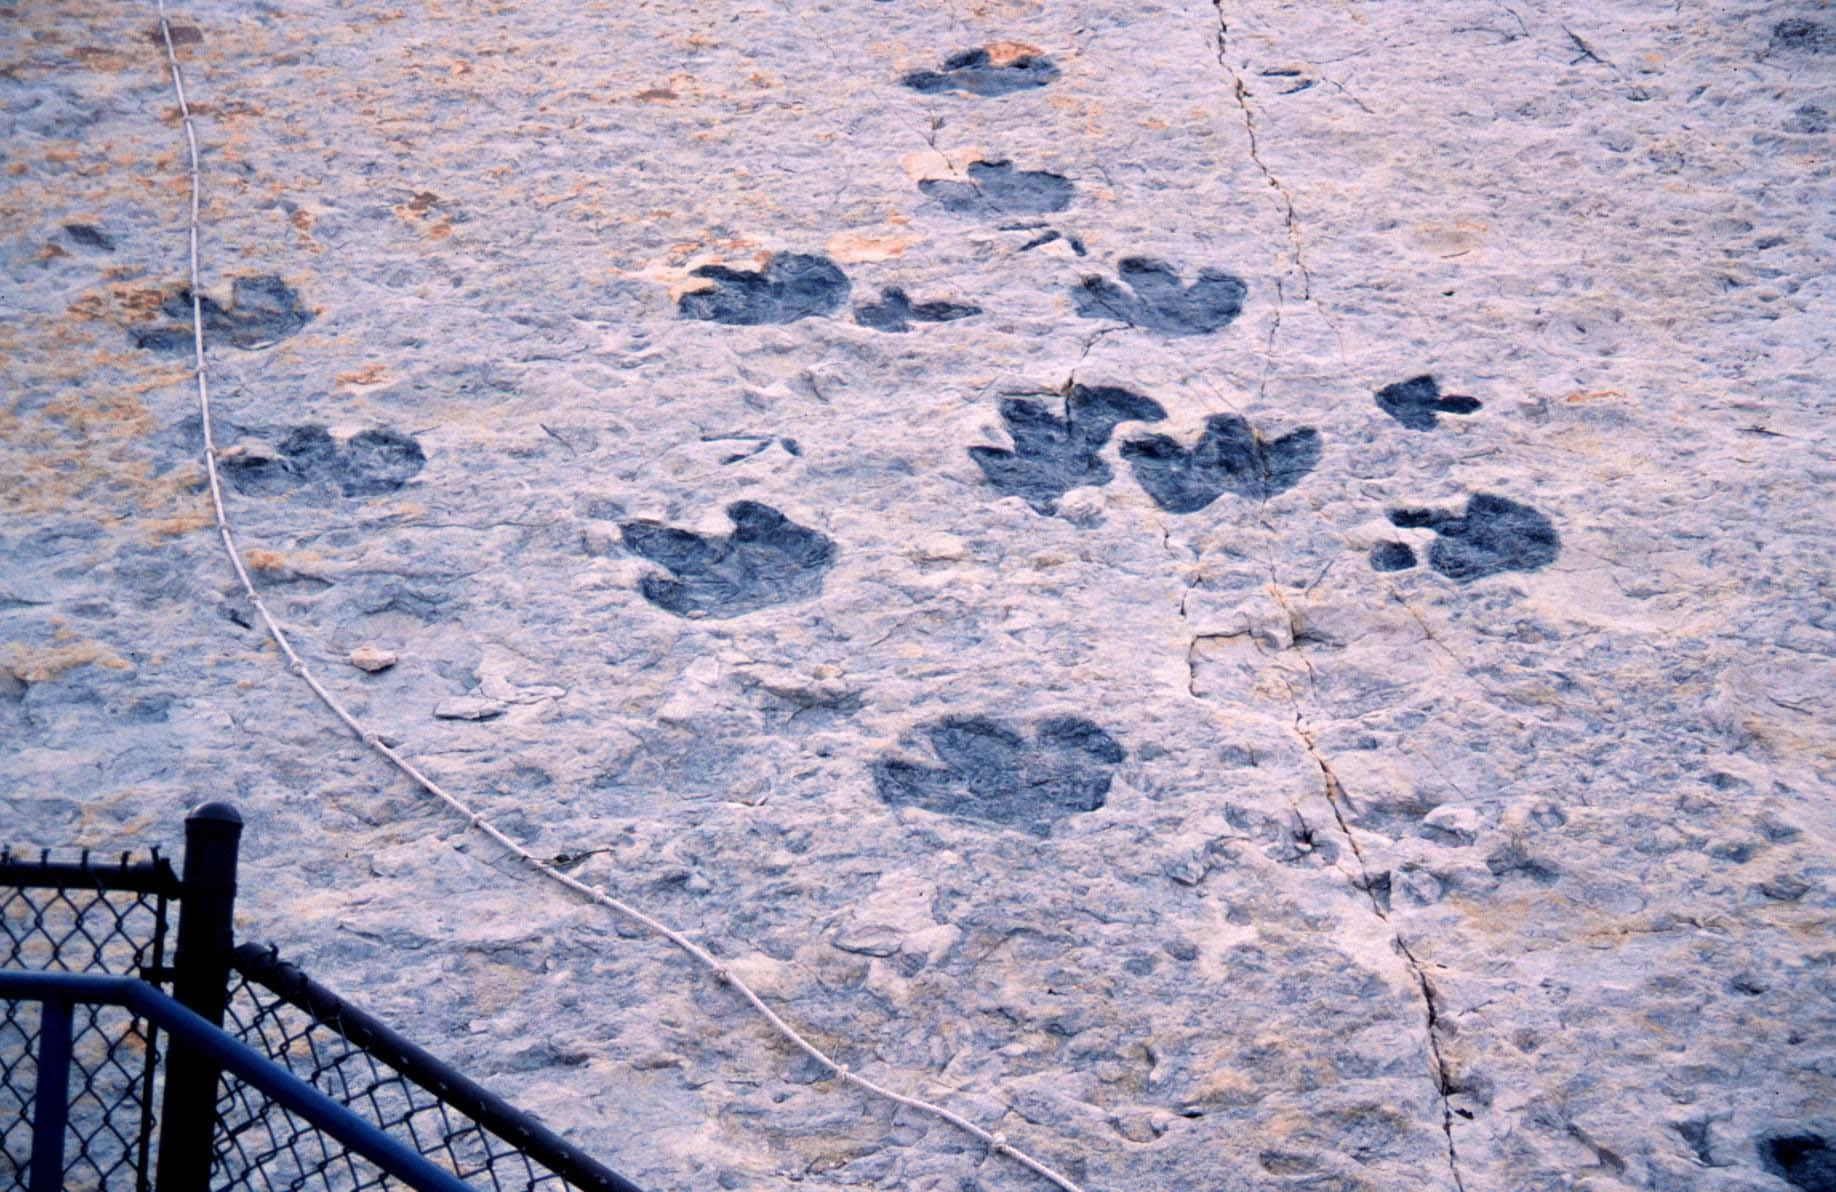
\includegraphics[width=0.62\linewidth]{images/book1/g7-dinosaur-tracks.jpg}

{\small कोलोराडो (संयुक्त राज्य अमेरिका) में मॉरिसन के पास डायनासोर रिज पर डायनासोर
के पैरों के निशान: नरम ज़मीन पर छूटे दर्जनों निशान, अब \omterm{def:g3:stones-pebbles-sand:rock}{चट्टान} की एक झुकी हुई सतह।
ज़्यादातर पौधे खाने वाले डायनासोरों ने बनाए, कुछ पतली उँगलियों वाले मांसाहारी
डायनासोरों ने। फ़ोटो: डेक्स्टर पर्किन्स (CC0, विकिमीडिया
कॉमन्स के ज़रिए)।}
% ledger: commons:dino-tracks
\label{fig:g7:sediments-and-fossils:tracks}
\end{omfigure}

जीव विज्ञान जीवों के लंबे इतिहास का पीछा करने के लिए \omterm{def:g7:sediments-and-fossils:fossil}{जीवाश्मों} का उपयोग करता है।
इस किताब में \omterm{def:g7:sediments-and-fossils:fossil}{जीवाश्म} दूसरी तरह के सुराग हैं: वे हमें बताते हैं कि जब वह जानवर वहाँ
रहता था, तब वह जगह कैसी थी।

\section{परतें और जीवाश्म, अतीत का एक अभिलेख}

हर परत उस जगह के निशान सँजोकर रखती है जहाँ वह बिछी थी। प्रवाल की भित्तियाँ आज
गरम, साफ़, उथले \omterm{def:g2:water-on-earth:ocean}{समुद्रों} में बढ़ती हैं; तरंग-चिह्न उथले पानी में, \omterm{def:g1:landscapes-around-us:water}{झील}, \omterm{def:g1:landscapes-around-us:water}{नदी} या
\omterm{def:g2:water-on-earth:ocean}{समुद्र} के किनारे, \omterm{def:g3:stones-pebbles-sand:sand}{रेत} पर बनते हैं; कोयला प्राचीन जंगलों और दलदलों के पौधों से बना;
ब्रैकियोपॉड, क्रिनॉइड और ट्राइलोबाइट केवल \omterm{def:g2:water-on-earth:ocean}{समुद्र} में रहते थे। जब यही सुराग किसी पुरानी परत में मिलते हैं, तो वह जगह
शायद परत बनते समय वैसी ही थी।
% ledger: noaa:coral-where, nps:ripple-marks, nps:ripples-shallow, usgs:coal-origin, nps:trilobite

\begin{center}
\small
\begin{tabular}{|p{0.36\linewidth}|p{0.52\linewidth}|}
\hline
\textbf{परत में सुराग} & \textbf{परत बनते समय वह जगह} \\
\hline
प्रवाल & एक गरम, उथला, साफ़ \omterm{def:g2:water-on-earth:ocean}{समुद्र} \\
\hline
समुद्री जानवरों की सीपियाँ (ब्रैकियोपॉड, क्रिनॉइड, ट्राइलोबाइट) & एक \omterm{def:g2:water-on-earth:ocean}{समुद्र} \\
\hline
किसी परत की सतह पर तरंग-चिह्न & उथला पानी, \omterm{def:g1:landscapes-around-us:water}{झील}, \omterm{def:g1:landscapes-around-us:water}{नदी} या \omterm{def:g2:water-on-earth:ocean}{समुद्र} के किनारे \\
\hline
पैरों के निशान & नरम, गीला \omterm{def:g3:stones-pebbles-sand:sand}{कीचड़} या \omterm{def:g3:stones-pebbles-sand:sand}{रेत}, अक्सर किसी \omterm{def:g1:landscapes-around-us:water}{तट} या \omterm{def:g1:landscapes-around-us:water}{नदी} के किनारे पर \\
\hline
कोयला & एक दलदली जंगल या दलदल \\
\hline
पत्तियाँ और व्याध पतंगे के पंख & ज़मीन, जिस पर पौधे उगते हों \\
\hline
\end{tabular}
\end{center}
% ledger: noaa:coral-where, nps:grca-fossils, nps:trilobite, nps:ripple-marks, nps:ripples-shallow, ucmp:footprints, usgs:coal-origin

\begin{method}[एक परत को पढ़ना]\label{met:g7:sediments-and-fossils:reading}
\begin{enumerate}
  \item कणों को देखो: मोटे कण वहाँ बैठते हैं जहाँ पानी तेज़ चलता है, महीन \omterm{def:g3:stones-pebbles-sand:sand}{कीचड़}
        केवल वहाँ जहाँ वह शांत है।
  \item \omterm{def:g7:sediments-and-fossils:fossil}{जीवाश्म} और निशान ढूँढो (प्रवाल, सीपियाँ, पैरों के निशान, तरंग-चिह्न,
        पौधों के अवशेष, कोयला) और ऊपर की तालिका का उपयोग करो।
  \item सुरागों को जोड़कर उस जगह की एक तस्वीर बनाओ: ज़मीन या \omterm{def:g2:water-on-earth:ocean}{समुद्र}, उथला या
        गहरा, शांत या बहता पानी।
\end{enumerate}
\end{method}

\begin{omfigure}
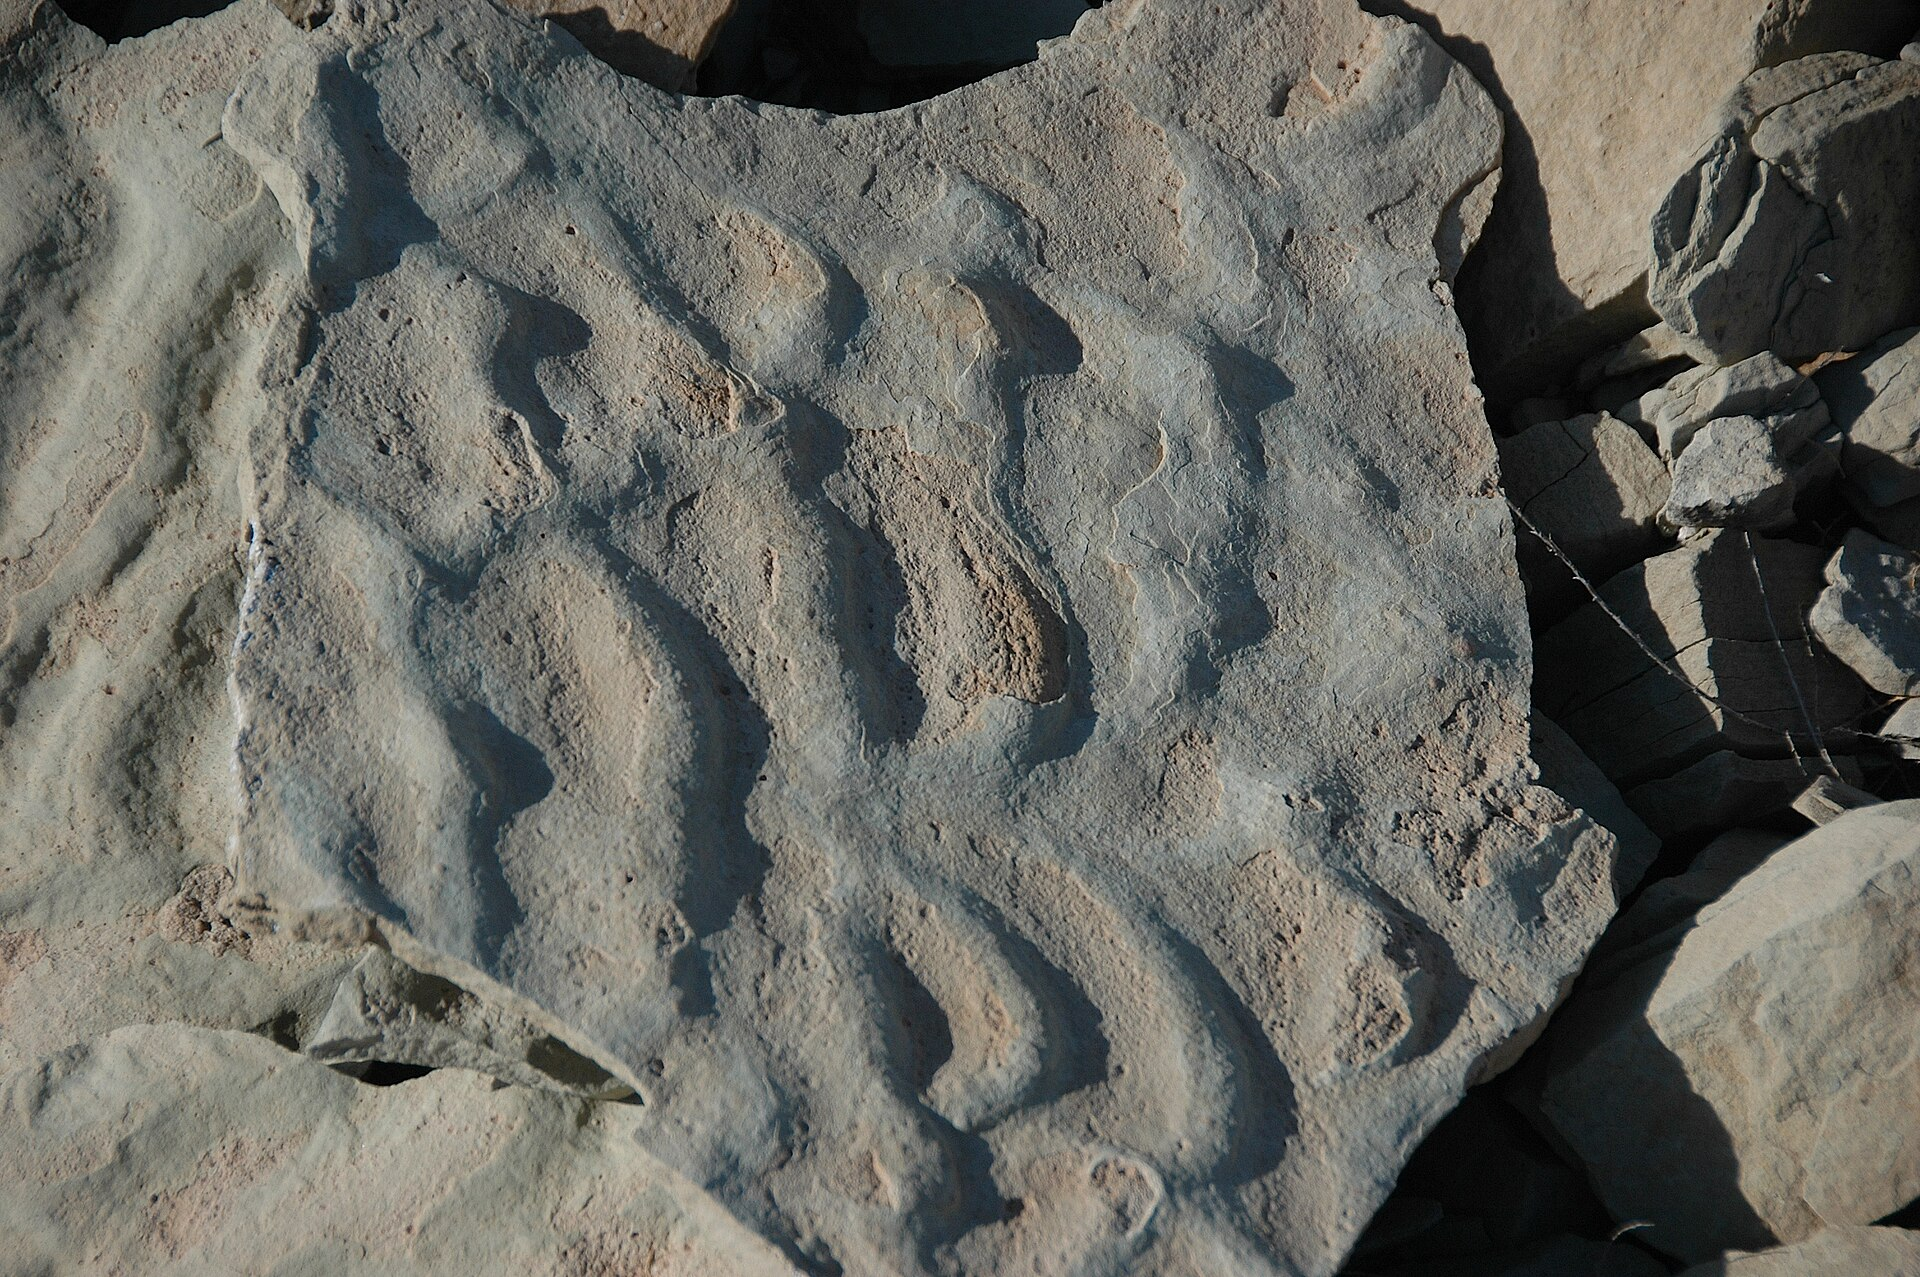
\includegraphics[width=0.56\linewidth]{images/book1/g7-ripple-marks.jpg}

{\small यूटा (संयुक्त राज्य अमेरिका) के कैपिटल रीफ़ राष्ट्रीय उद्यान में बलुआ पत्थर की
एक पटिया पर तरंग-चिह्न: \omterm{def:g3:stones-pebbles-sand:sand}{रेत} को कभी बहते पानी ने लहरदार बनाया था, आज के किसी \omterm{def:g2:water-on-earth:ocean}{समुद्र}
\omterm{def:g1:landscapes-around-us:water}{तट} या नाले के तल की \omterm{def:g3:stones-pebbles-sand:sand}{रेत} की तरह। फ़ोटो: जेम्स
सेंट~जॉन (CC BY 2.0, विकिमीडिया कॉमन्स के ज़रिए)।}
% ledger: commons:ripples, nps:ripple-marks
\label{fig:g7:sediments-and-fossils:ripples}
\end{omfigure}

\begin{example}[ग्रैंड कैन्यन का शिखर]\label{ex:g7:sediments-and-fossils:kaibab}
ग्रैंड कैन्यन की सबसे ऊपरी परत, काइबाब चूना पत्थर, ब्रैकियोपॉड की सीपियों और
क्रिनॉइड के तने के टुकड़ों से भरी है, जो दोनों समुद्री जानवर हैं। वह एक \omterm{def:g2:water-on-earth:ocean}{समुद्र} की तली
पर बनी। आज वही परत \omterm{def:g4:world-physical-map:altitude}{समुद्र तल} से लगभग \qty{2700}{m} (\num{9000}~फ़ुट) तक ऊपर है:
उसके बनने के बाद पूरा क्षेत्र ऊपर
उठा है।
% ledger: nps:grca-fossils, nps:grca-kaibab
\end{example}

परतों के ढेर को एक \emph{स्तंभ} के रूप में बनाया जा सकता है: परतें उसी क्रम में
रखी हुईं जिसमें वे बनीं, उनकी मोटाई पैमाने पर, और उनके सुराग बगल में लिखे हुए।
वार्डन पहाड़ियों का स्तंभ, जो इस शृंखला के अभ्यासों का काल्पनिक क्षेत्र है,
नीचे है।

\begin{omfigure}
\begin{tikzpicture}
  \begin{axis}[width=4.2cm, height=9.2cm, scale only axis=false, xmin=0, xmax=1, ymin=-60, ymax=485,
      axis x line=none, axis y line*=left, ytick={0,100,200,300,400},
      ylabel={बलुआ पत्थर के आधार से ऊपर मीटर}, label style={font=\footnotesize},
      tick label style={font=\scriptsize}, clip=false]
    \addplot[lith schist, draw=black!70, line width=0.3pt] table {figdata/out/grade-7-varden_column-unit-older.dat};
    \addplot[lith sandstone, draw=black!70, line width=0.3pt] table {figdata/out/grade-7-varden_column-unit-sandstone.dat};
    \addplot[lith limestone, draw=black!70, line width=0.3pt] table {figdata/out/grade-7-varden_column-unit-limestone.dat};
    \addplot[lith shale, draw=black!70, line width=0.3pt] table {figdata/out/grade-7-varden_column-unit-shale.dat};
    \addplot[om lith={white}{om limestone}, draw=black!70, line width=0.3pt] table {figdata/out/grade-7-varden_column-unit-chalk.dat};
    \node[anchor=west, align=left, font=\footnotesize] at (axis cs:1.12,450) {\textbf{खड़िया}: उसका ऊपरी हिस्सा\\घिसकर हट गया है (केवल आधार बना है)};
    \node[anchor=west, align=left, font=\footnotesize] at (axis cs:1.12,350) {\textbf{शेल}, \qty{100}{m}: बहुत महीन कण;\\अमोनाइट};
    \node[anchor=west, align=left, font=\footnotesize] at (axis cs:1.12,210) {\textbf{चूना पत्थर}, \qty{180}{m}:\\प्रवाल और सीपियाँ};
    \node[anchor=west, align=left, font=\footnotesize] at (axis cs:1.12,60) {\textbf{बलुआ पत्थर}, \qty{120}{m}:\\तरंग-चिह्न, पैरों के निशान};
    \node[anchor=west, align=left, font=\footnotesize] at (axis cs:1.12,-30) {पुरानी चट्टानें (शिस्ट और ग्रेनाइट),\\बलुआ पत्थर आने से पहले घिसकर समतल};
  \end{axis}
\end{tikzpicture}

\medskip
{\small वार्डन पहाड़ियों का स्तंभ, इस शृंखला का काल्पनिक क्षेत्र: परतें उसी क्रम में
जिसमें वे बनीं, पहली सबसे नीचे, उनकी मोटाई पैमाने पर। बगल में लिखे \omterm{def:g7:sediments-and-fossils:fossil}{जीवाश्म} और
निशान अभ्यास के आँकड़े
हैं।}
% ledger: (invented region: figdata/shared/region.py, drawn by figdata/grade-7/varden_column.py)
\label{fig:g7:sediments-and-fossils:column}
\end{omfigure}

\begin{omfigure}
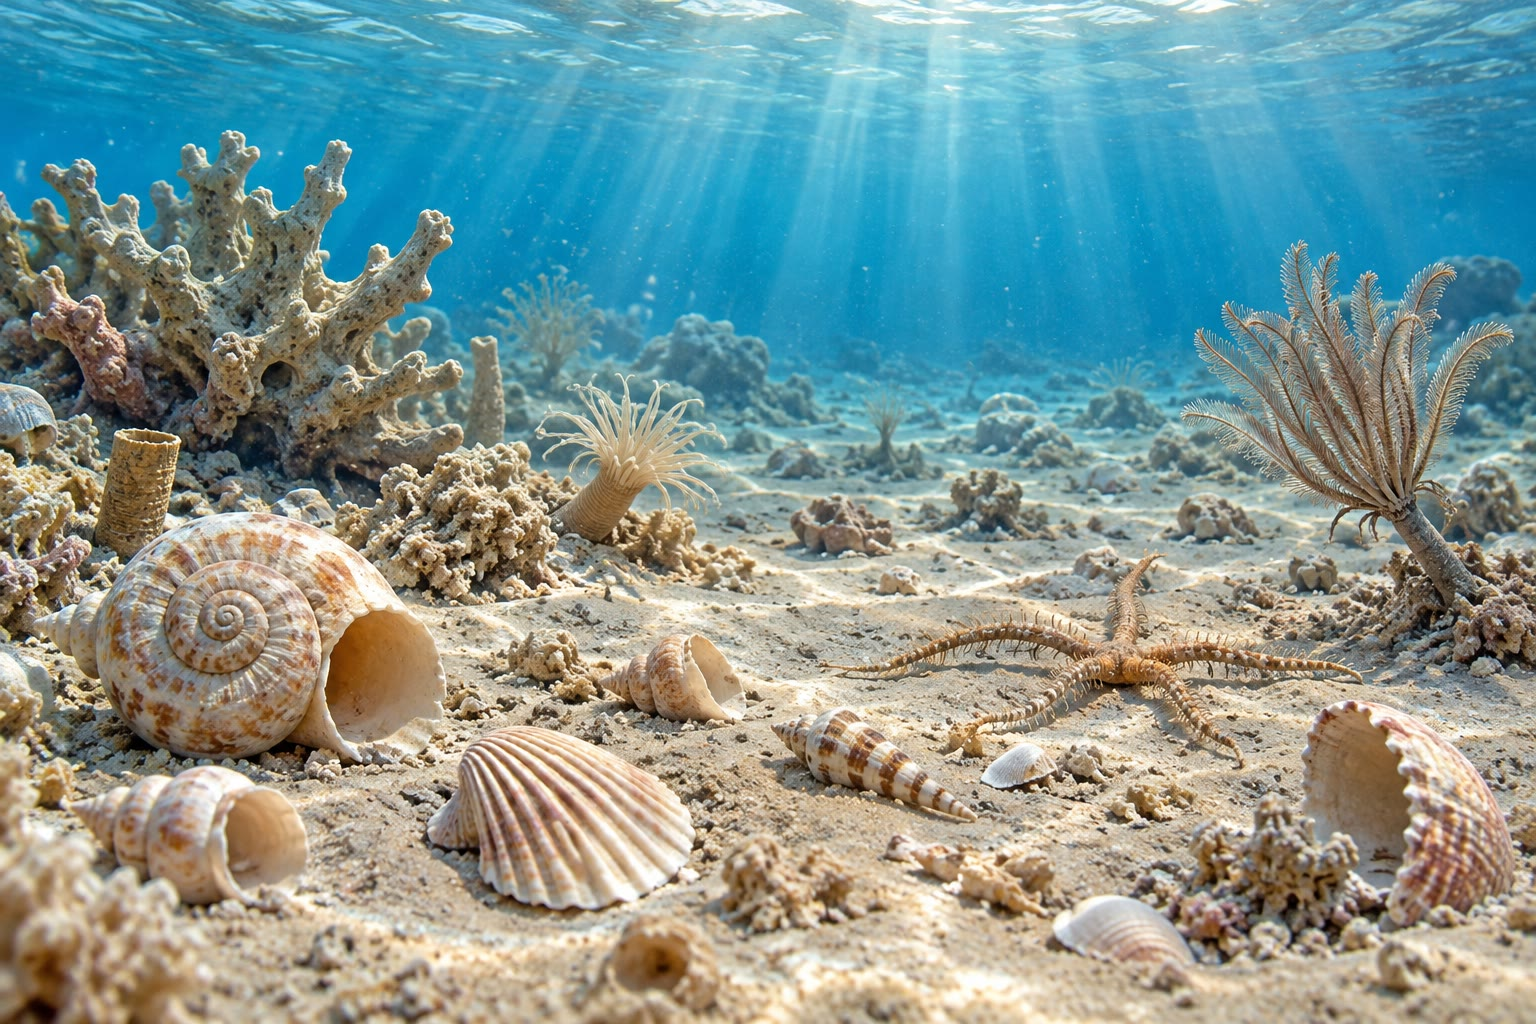
\includegraphics[width=0.6\linewidth]{images/book1/ai/g7-shallow-sea.jpg}

{\small बहुत पहले का एक गरम, उथला समुद्री तल, जैसा वह तब दिखता होगा जब सीपियाँ और
प्रवाल के टुकड़े भविष्य के एक चूना पत्थर में बैठ रहे थे (एक सामान्य दृश्य का
AI चित्रण)।}
\label{fig:g7:sediments-and-fossils:shallow-sea}
\end{omfigure}

\begin{remark}[देखो, फ़ोटो लो, वहीं छोड़ दो]\label{rem:g7:sediments-and-fossils:leave}
बहुत-सी संरक्षित जगहों पर \omterm{def:g7:sediments-and-fossils:fossil}{जीवाश्म} ले जाना मना है: उदाहरण के लिए, ग्रैंड कैन्यन में
किसी भी \omterm{def:g7:sediments-and-fossils:fossil}{जीवाश्म} को खोदना, हिलाना या ले जाना क़ानून के ख़िलाफ़ है। जिस पर्यटक को
कोई \omterm{def:g7:sediments-and-fossils:fossil}{जीवाश्म} मिलता है, वह फ़ोटो लेता है या चित्र बनाता है, उसे वहीं छोड़ देता है
ताकि दूसरे देख सकें और वैज्ञानिक उसका अध्ययन कर सकें, और किसी रेंजर को
बताता है।
\end{remark}
% ledger: nps:grca-fossils

\begin{inthefield}[आज बिछते अवसाद]
किसी \omterm{def:g2:water-on-earth:ocean}{समुद्र} \omterm{def:g1:landscapes-around-us:water}{तट}, \omterm{def:g1:landscapes-around-us:water}{झील} के किनारे या नाले के किनारे पर, किसी बड़े के साथ, उथले पानी के
नीचे की \omterm{def:g3:stones-pebbles-sand:sand}{रेत} देखो: बहता पानी उसे लहरों जैसा आकार देता है, उन लहरों जैसा जो पुराने
बलुआ पत्थर में सुरक्षित हैं। पानी के किनारे के पास गीली \omterm{def:g3:stones-pebbles-sand:sand}{रेत} पर अपने पैर का एक निशान
छोड़ो और देखो कि अगली लहरें उसके साथ क्या करती हैं। \omterm{def:g4:clouds-rain-snow:precipitation}{बारिश} वाले दिन के बाद, सूख चुके
किसी डबरे को देखो: उसकी तली की \omterm{def:g3:stones-pebbles-sand:sand}{रेत} पर अक्सर महीन \omterm{def:g3:stones-pebbles-sand:sand}{कीचड़} की एक पतली परत होती है ---
सबसे महीन कण सबसे आख़िर में बैठे, जब पानी स्थिर था। जो देखो उसका चित्र बनाओ, और
लिखो कि कहाँ और
कब।
\end{inthefield}
% ledger: nps:ripple-marks, ucmp:footprints, usgs:strata

\section{अभ्यास}

\begin{exercise}[$\star$]\label{exo:g7:sediments-and-fossils:1}
हर शब्द को उसके अर्थ से मिलाओ: \omterm{def:g7:sediments-and-fossils:sediment}{अवसाद}; \omterm{def:g7:sediments-and-fossils:layer}{स्तर}; \omterm{def:g7:sediments-and-fossils:fossil}{जीवाश्म}; \omterm{def:g7:sediments-and-fossils:fossil}{साँचा}; \omterm{def:g7:sediments-and-fossils:fossil}{ढलाई}; \omterm{def:g7:sediments-and-fossils:fossil}{चिह्न जीवाश्म}।
(क) \omterm{def:g3:stones-pebbles-sand:rock}{चट्टान} में बची एक खोखली जगह जहाँ कोई सीपी घुल गई हो। (ख) \omterm{def:g3:stones-pebbles-sand:rock}{चट्टान} में सुरक्षित
पैरों का निशान या बिल। (ग) पानी, हवा या बर्फ़ द्वारा बिछाया गया ढीला पदार्थ।
(घ) किसी खोखली जगह के \omterm{def:g6:rocks-and-minerals:mineral}{खनिजों} से भरने पर बना पत्थर का प्रतिरूप। (ङ) एक ही समय में
बिछी \omterm{def:g7:sediments-and-fossils:sediment}{अवसाद} की एक चादर। (च) बहुत पहले के किसी जीव के अवशेष या निशान, जो \omterm{def:g3:stones-pebbles-sand:rock}{चट्टान} में
सुरक्षित हों।
\end{exercise}

\begin{exercise}[$\star$]\label{exo:g7:sediments-and-fossils:2}
यह बताने के लिए कि सतह पर मिलने वाली एक सीपी \omterm{def:g7:sediments-and-fossils:fossil}{जीवाश्म} कैसे बनती है, इन चरणों को
क्रम में रखो: (क) \omterm{def:g5:water-shapes-the-land:erosion}{अपरदन} उसके ऊपर की परतों को घिस देता है; (ख) जानवर \omterm{def:g2:water-on-earth:ocean}{समुद्र} की
तली पर मरता है; (ग) नई परतें जमा होती हैं और सीपी पत्थर बन जाती है; (घ) \omterm{def:g3:stones-pebbles-sand:sand}{कीचड़}
सीपी को जल्दी ढक लेता है।
\end{exercise}

\begin{exercise}[$\star$]\label{exo:g7:sediments-and-fossils:3}
सुरागों वाली तालिका का उपयोग करो। हर परत कहाँ बनी? (क) प्रवालों से भरा एक चूना
पत्थर। (ख) एक बलुआ पत्थर जिसकी सतह पर तरंग-चिह्न हैं। (ग) कोयले की एक गहरी परत।
(घ) पत्तियों की छाप और एक व्याध पतंगे के पंख वाला एक शेल।
\end{exercise}

\begin{exercise}[$\star$]\label{exo:g7:sediments-and-fossils:4}
सही या ग़लत? ग़लत वाक्यों को सुधारो। (क) मरने वाला हर जानवर एक दिन \omterm{def:g7:sediments-and-fossils:fossil}{जीवाश्म} बनता
है। (ख) पैर का निशान \omterm{def:g7:sediments-and-fossils:fossil}{जीवाश्म} हो सकता है। (ग) जब \omterm{def:g3:stones-pebbles-sand:sand}{कीचड़} भरा पानी धीमा होता है, तो
महीन \omterm{def:g3:stones-pebbles-sand:sand}{कीचड़} पहले बैठता है। (घ) \omterm{def:g7:sediments-and-fossils:sediment}{अवसाद} समतल
बिछते हैं।
\end{exercise}

\begin{exercise}[$\star\star$]\label{exo:g7:sediments-and-fossils:5}
वार्डन पहाड़ियों के स्तंभ का उपयोग करो। (क) बलुआ पत्थर, चूना पत्थर और शेल की
मोटाई बताओ। (ख) उनकी कुल मोटाई कितनी है? (ग) इस कुल का कितना प्रतिशत चूना
पत्थर है? निकटतम पूर्ण संख्या तक पूर्णांकित करो। (घ) स्तंभ खड़िया की कोई मोटाई
क्यों नहीं देता?
\end{exercise}

\begin{exercise}[$\star\star$]\label{exo:g7:sediments-and-fossils:6}
एक विद्यार्थी \omterm{def:g3:stones-pebbles-sand:pebble}{बजरी}, \omterm{def:g3:stones-pebbles-sand:sand}{रेत} और \omterm{def:g3:stones-pebbles-sand:sand}{कीचड़} वाले पानी के एक मर्तबान को हिलाती है, और उसे
बैठने देती है। (क) अगले दिन का मर्तबान बनाओ, और परतों के नाम लिखो। (ख) एक घंटे
बाद भी पानी गदला क्यों है? (ग) वह फिर \omterm{def:g3:stones-pebbles-sand:sand}{रेत} और \omterm{def:g3:stones-pebbles-sand:sand}{कीचड़} डालती है और उसे बैठने देती है।
अब उसे तली पर क्या दिखता है? (घ) मर्तबान की कौन-सी परत सबसे पहले
बनी?
\end{exercise}

\begin{exercise}[$\star\star$]\label{exo:g7:sediments-and-fossils:7}
इनमें से किसके \omterm{def:g7:sediments-and-fossils:fossil}{जीवाश्म} बनने की संभावना सबसे ज़्यादा है, और किसकी सबसे कम? समझाओ।
(क) पथरीले \omterm{def:g1:landscapes-around-us:water}{तट} पर बहकर आई एक जेलीफ़िश। (ख) शांत \omterm{def:g1:landscapes-around-us:water}{झील} के \omterm{def:g3:stones-pebbles-sand:sand}{कीचड़} में दबा घोंघे का
खोल। (ग) किसी सूखे \omterm{def:g1:landscapes-around-us:landform}{मैदान} पर वर्षों पड़ी एक हड्डी। (घ) \omterm{def:g1:landscapes-around-us:water}{नदी} की \omterm{def:g5:water-shapes-the-land:flood}{बाढ़} में \omterm{def:g3:stones-pebbles-sand:sand}{रेत} से ढकी
सीप की एक सीपी।
\end{exercise}

\begin{exercise}[$\star\star$]\label{exo:g7:sediments-and-fossils:8}
एक सीपी \omterm{def:g3:stones-pebbles-sand:sand}{रेत} में दबी है जो बलुआ पत्थर बन जाती है। \omterm{def:g3:stones-pebbles-sand:rock}{चट्टान} में से रिसता पानी सीपी को
पूरी तरह घोल देता है। (क) \omterm{def:g3:stones-pebbles-sand:rock}{चट्टान} में क्या बचता है? (ख) बाद में \omterm{def:g6:rocks-and-minerals:mineral}{खनिज} इस खोखली जगह
को भर देते हैं। क्या बनता है? (ग) क्या सीपी ख़ुद अब भी वहाँ है? (घ) \omterm{def:g7:sediments-and-fossils:fossil}{साँचे} और
ढलाइयाँ शेल की तुलना में बलुआ पत्थर में ज़्यादा क्यों मिलती हैं? (सोचो कि कणों के
बीच से पानी कितनी आसानी से गुज़रता है।)
\end{exercise}

\begin{exercise}[$\star\star$]\label{exo:g7:sediments-and-fossils:9}
ग्रैंड कैन्यन औसतन \qty{1.6}{km} गहरा है। (क) यह गहराई मीटर में लिखो। (ख) मान लो
कैन्यन की दीवारें \qty{80}{m} मोटी परतों से बनी होतीं: किनारे से तली तक कितनी परतें
समातीं? (ग) \qty{160}{m} की परत गहराई का
कितना प्रतिशत है?
\end{exercise}

\begin{exercise}[$\star\star$]\label{exo:g7:sediments-and-fossils:10}
एक बलुआ पत्थर में डायनासोर के पैरों के निशान मिलते हैं। (क) क्या डायनासोर सख़्त
\omterm{def:g3:stones-pebbles-sand:rock}{चट्टान} पर चल रहे थे? समझाओ। (ख) \omterm{def:g3:stones-pebbles-sand:sand}{कीचड़} भरे \omterm{def:g1:landscapes-around-us:water}{तट} पर छूटे ज़्यादातर निशान क्यों मिट
जाते हैं? (ग) निशानों के सुरक्षित रहने के लिए डायनासोरों के गुज़रने के जल्दी बाद क्या
होना ज़रूरी था? (घ) पैर का निशान शरीर \omterm{def:g7:sediments-and-fossils:fossil}{जीवाश्म} है या
\omterm{def:g7:sediments-and-fossils:fossil}{चिह्न जीवाश्म}?
\end{exercise}

\begin{exercise}[$\star\star\star$]\label{exo:g7:sediments-and-fossils:11}
एक \omterm{def:g1:landscapes-around-us:water}{झील} में हर \omterm{def:g5:water-shapes-the-land:flood}{बाढ़} लगभग \qty{2}{cm} मोटी \omterm{def:g3:stones-pebbles-sand:sand}{रेत} की एक परत छोड़ती है, और उसके बाद के
शांत हफ़्ते लगभग \qty{5}{mm} मोटी \omterm{def:g3:stones-pebbles-sand:sand}{कीचड़} की एक परत (अभ्यास के आँकड़े)। (क) परतों
की एक जोड़ी मिलीमीटर में कितनी मोटी है? (ख) \omterm{def:g1:landscapes-around-us:water}{झील} की तली से निकाला गया एक कोर
\qty{1}{m} लंबा है और केवल ऐसी जोड़ियों से बना है। वह कितनी \omterm{def:g5:water-shapes-the-land:flood}{बाढ़ों} को दर्ज करता है?
(ग) \omterm{def:g1:landscapes-around-us:water}{नदी} के \omterm{def:g5:water-shapes-the-land:source-mouth}{मुहाने} के पास \omterm{def:g3:stones-pebbles-sand:sand}{रेत} की परतें ज़्यादा मोटी हैं, दूर वे पतली हैं। समझाओ
क्यों। (घ) \omterm{def:g5:water-shapes-the-land:source-mouth}{मुहाने} से दूर \omterm{def:g3:stones-pebbles-sand:sand}{रेत} से ज़्यादा \omterm{def:g3:stones-pebbles-sand:sand}{कीचड़}
क्यों है?
\end{exercise}

\begin{exercise}[$\star\star\star$]\label{exo:g7:sediments-and-fossils:12}
\omterm{def:g3:stones-pebbles-sand:rock}{चट्टानों} में मिलने वाले \omterm{def:g7:sediments-and-fossils:fossil}{जीवाश्म} ज़्यादातर सीपियाँ और नन्हे अवशेष हैं; नरम जानवरों के
\omterm{def:g7:sediments-and-fossils:fossil}{जीवाश्म} दुर्लभ हैं, और डायनासोर सभी \omterm{def:g7:sediments-and-fossils:fossil}{जीवाश्मों} का केवल एक बहुत छोटा हिस्सा हैं।
(क) समझाओ कि सीपियाँ इतनी आम क्यों हैं। (ख) समझाओ कि नरम जानवर दुर्लभ क्यों हैं।
(ग) एक वैज्ञानिक उन सभी जानवरों को जानना चाहती है जो किसी प्राचीन \omterm{def:g2:water-on-earth:ocean}{समुद्र} में रहते
थे। क्या \omterm{def:g7:sediments-and-fossils:fossil}{जीवाश्म} पूरी सूची दे सकते हैं? समझाओ।
\end{exercise}

\section{समस्या: वार्डन पहाड़ियों का स्तंभ}

\begin{problem}[{सप्ताहांत समस्या --- वार्डन पहाड़ियों की परतें एक-एक करके पढ़ी जाती
हैं, उनके जीवाश्म बताते हैं कि वे कहाँ बनीं, और चूना पत्थर के जमने में लगा समय
निकाला जाता है}]
\label{pb:g7:sediments-and-fossils:1}
% ledger: (invented region: figdata/shared/region.py; rates are exercise data, figdata/grade-7/varden_column.py part rates)
इस अध्याय के वार्डन पहाड़ियों के स्तंभ का उपयोग करो। उसके बलुआ पत्थर में तरंग-चिह्न
और पैरों के निशान हैं; उसके चूना पत्थर में प्रवाल और सीपियाँ हैं; उसका शेल बहुत
महीन कणों से बना है, अमोनाइट के साथ; सबसे ऊपर की खड़िया आंशिक रूप से घिसकर हट
गई है।

\medskip
\noindent\textbf{भाग I --- परतों को पढ़ना।}\par\nopagebreak
\begin{enumerate}[beginpenalty=10000]
  \item चारों परतों की सूची बनाओ, सबसे पहले बिछी परत से आख़िरी तक।
  \item बलुआ पत्थर, चूना पत्थर और शेल की मोटाई बताओ, और उनका
        कुल योग।
  \item इस कुल का कितना प्रतिशत चूना पत्थर है?
  \item कोई यह क्यों नहीं बता सकता कि बनते समय खड़िया कितनी मोटी थी?
\end{enumerate}

\medskip
\noindent\textbf{भाग II --- उनमें के जीवाश्म।}\par\nopagebreak
\begin{enumerate}[resume, beginpenalty=10000]
  \item बलुआ पत्थर कहाँ बना? दो सुराग बताओ।
  \item चूना पत्थर कहाँ बना? सुराग बताओ।
  \item शेल बहुत महीन कणों से बना है। जब वह बिछा, तब पानी शांत था या बहता हुआ?
        समझाओ।
  \item बलुआ पत्थर से शेल तक, तीन वाक्यों में उस जगह की कहानी
        बताओ।
\end{enumerate}

\medskip
\noindent\textbf{भाग III --- इसमें कितना समय लगा।}\par\nopagebreak
\begin{enumerate}[resume, beginpenalty=10000]
  \item चूना पत्थर की मोटाई सेंटीमीटर में लिखो।
  \item मान लो बलुआ पत्थर हर 20 वर्ष में \qty{1}{cm} जमा हुआ। उसके \qty{120}{m} में
        कितने वर्ष लगे?
  \item मान लो चूना पत्थर हर 100 वर्ष में \qty{1}{cm} जमा हुआ।
        \qty{1}{m} चूना पत्थर में कितने वर्ष लगे?
  \item \qty{180}{m} चूना पत्थर में कितने वर्ष लगे? यह बलुआ पत्थर से कितने गुना
        ज़्यादा है?
\end{enumerate}
\end{problem}
